%%%%%%%%%%%%%%%%%%%%%%%%%%%%%%%%%%%%%%%%%
% Memo
% LaTeX Template
% Version 1.0 (30/12/13)
%
% This template has been downloaded from:
% http://www.LaTeXTemplates.com
%
% Original author:
% Rob Oakes (http://www.oak-tree.us) with modifications by:
% Vel (vel@latextemplates.com)
%
% License:
% CC BY-NC-SA 3.0 (http://creativecommons.org/licenses/by-nc-sa/3.0/)
%
%%%%%%%%%%%%%%%%%%%%%%%%%%%%%%%%%%%%%%%%%

\documentclass[letterpaper,11pt]{texMemo} % Set the paper size (letterpaper, a4paper, etc) and font size (10pt, 11pt or 12pt)

\usepackage{parskip} % Adds spacing between paragraphs
\setlength{\parindent}{15pt} % Indent paragraphs
\usepackage{censor}

\usepackage{hyperref}
\hypersetup{
colorlinks=true,
linkcolor=blue,
filecolor=magenta,      
urlcolor=blue,
citecolor=blue,
}

%----------------------------------------------------------------------------------------
%	MEMO INFORMATION
%----------------------------------------------------------------------------------------

\memoto{\blackout{Xxxxxxxx Xxxxxxxx xxx Xxxxxx Xxxxxxx}} % Recipient(s)

\memofrom{Michael Brodskiy} % Sender(s)

\memosubject{Research Synthesis and Annotated Bibliography Peer Review} % Memo subject

\memodate{Wednesday, May 29, 2024} % Date, set to \today for automatically printing todays date

\logo{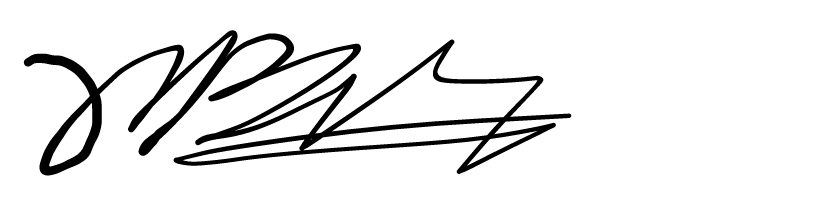
\includegraphics[width=0.3\textwidth]{logo.png}} % Institution logo at the top right of the memo, comment out this line for no logo

%----------------------------------------------------------------------------------------

\begin{document}

\maketitle % Print the memo header information

%----------------------------------------------------------------------------------------
%	MEMO CONTENT
%----------------------------------------------------------------------------------------

This document was quite an interesting read! I particularly enjoyed the juxtaposition of the energy center size requirements to the country of Ireland, as it added a clear sense of urgency by putting the problem into perspective.

Looking at the annotated bibliography, all of the sources seem to be directly pertinent to the topic at hand. I would, however, recommend that, when summarizing the argument of a publication, try starting with something along the lines of "the document \textit{argues} . . ." or "this publication \textit{considers} . . ." instead of more mundanely stating "this paper is important because . . ." In doing so, it more clearly differentiates your own synthesis and opinions regarding the document from the author's findings. There are also a few typos strewn throughout like: "Universit\textbf{y} of Massachusetts" and "minimise" to "minimi\textbf{z}e" (there may be others, so please consider reviewing once again). Other than this, I commend you for using quality sources and synthesizing them to find interesting solutions to a relevant problem.

As for the substance of the paper, you do a great job of defining acronyms before first use, like artificial intelligence (AI) and machine learning (ML). Oftentimes, technical writing novices forget to do this. Reading the entirety of the paper, I now understand that not only is AI and ML already creating a huge environmental impact with data centers, but this strain is also increasing; however, the future does seem optimistic, as the heat produced as a byproduct may be used for a specific purpose (like heating cities) by implementing heat pumps, rather than being released into the environment. The document does seem to perform quite a thoughtful synthesis; however, I would suggest one major update: beware of run-on sentences! There were many throughout, and, thus, consider proofreading and adding in more punctuation, when necessary.

In a more general scope, I would recommend that, in addition to using IEEE citation format, you would use an IEEE document format (an example can be found \href{https://www.IEEE.org/conference/publishing/templates.HTML}{here}). Using this would not only be beneficial for your future endeavors, but will also improve the overall readability of your exhibition. Also, a small fix would be to indent the first paragraph (to maintain conformity with the other paragraphs). Finally, I would also suggest getting rid of some of the citations. In general, when citing a work, it is unnecessary to re-cite it when continuing with the same thought (unless multiple documents are cited or a different document is cited before continuing).

Great work overall!

%----------------------------------------------------------------------------------------

\end{document}
